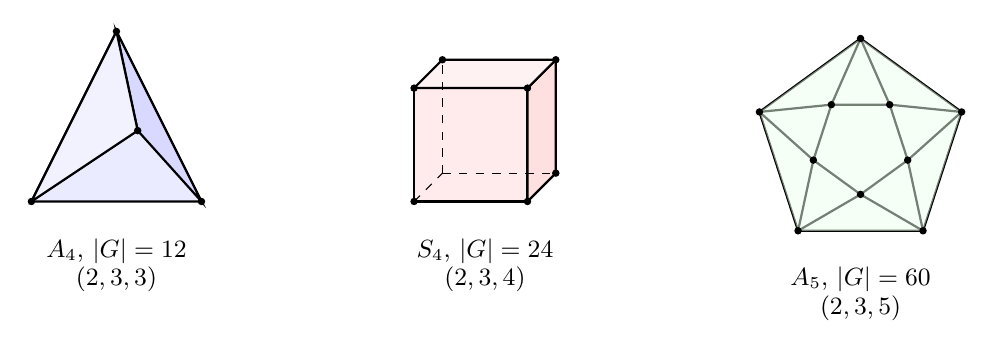
\begin{tikzpicture}[scale=0.9]
\begin{scope}[shift={(-5,0)}]
    \coordinate (A) at (0, 1.6);
    \coordinate (B) at (-1.2, -0.8);
    \coordinate (C) at (1.2, -0.8);
    \coordinate (D) at (0.3, 0.2);
    \draw[thick, fill=blue!8] (A) -- (B) -- (C) -- cycle;
    \draw[thick, fill=blue!15] (A) -- (C) -- (D) -- cycle;
    \draw[thick, fill=blue!5] (A) -- (B) -- (D) -- cycle;
    \draw[dashed, thin] (B) -- (D);
    \foreach \p in {A,B,C,D} \fill (\p) circle (1.5pt);
    \node at (0, -1.5) {\small \(A_4\), \(|G|=12\)};
    \node at (0, -1.9) {\small \((2,3,3)\)};
\end{scope}
\begin{scope}[shift={(0,0)}]
    \coordinate (A) at (-0.8, -0.8);
    \coordinate (B) at (0.8, -0.8);
    \coordinate (C) at (0.8, 0.8);
    \coordinate (D) at (-0.8, 0.8);
    \coordinate (E) at (-0.4, -0.4);
    \coordinate (F) at (1.2, -0.4);
    \coordinate (G) at (1.2, 1.2);
    \coordinate (H) at (-0.4, 1.2);
    \draw[thick, fill=red!8] (A) -- (B) -- (C) -- (D) -- cycle;
    \draw[thick, fill=red!12] (B) -- (F) -- (G) -- (C) -- cycle;
    \draw[thick, fill=red!5] (D) -- (C) -- (G) -- (H) -- cycle;
    \draw[dashed, thin] (A) -- (E);
    \draw[dashed, thin] (E) -- (F);
    \draw[dashed, thin] (E) -- (H);
    \foreach \p in {A,B,C,D,F,G,H} \fill (\p) circle (1.5pt);
    \node at (0.2, -1.5) {\small \(S_4\), \(|G|=24\)};
    \node at (0.2, -1.9) {\small \((2,3,4)\)};
\end{scope}
\begin{scope}[shift={(5.5,0)}]
    \foreach \i in {0,...,4} {
        \coordinate (O\i) at ({90+72*\i}:1.5);
    }
    \foreach \i in {0,...,4} {
        \coordinate (I\i) at ({90+72*\i+36}:0.7);
    }
    \draw[thick] (O0) -- (O1) -- (O2) -- (O3) -- (O4) -- cycle;
    \draw[thick] (I0) -- (I1) -- (I2) -- (I3) -- (I4) -- cycle;
    \foreach \i in {0,...,4} {
        \draw[thick] (O\i) -- (I\i);
        \pgfmathtruncatemacro{\j}{mod(\i+4,5)}
        \draw[thick] (O\i) -- (I\j);
    }
    \fill[green!8, opacity=0.5] (O0) -- (O1) -- (O2) -- (O3) -- (O4) -- cycle;
    \foreach \i in {0,...,4} \fill (O\i) circle (1.5pt);
    \foreach \i in {0,...,4} \fill (I\i) circle (1.5pt);
    \node at (0, -1.9) {\small \(A_5\), \(|G|=60\)};
    \node at (0, -2.3) {\small \((2,3,5)\)};
\end{scope}
\end{tikzpicture}
